\section{Work Process}

The Rapport and the product described in this rapport is created over the course of 12 weeks. I've decided due to the fact I'm working alone that I will not directly adapt a development method, as most of these build on the fact that you're working in teams. I will however work in iterations and in the beginning of each iteration adjust my schedule accordingly to my progress. I will be using kanbanflow as my main scheduling and time tracking system, as I've used this with big success before for smaller projects. My Initial schedule can be seen in \figref{fig:InitTimeplan} and we will look at what changes that have occurred in section \ref{ProjectPlanning}.

The 12 weeks available for this project have been split into 4 iteration of 3 weeks which each have a theme. Iteration 1 is where the introduction, setup and planning will happen for the most, iteration 2 have focus on technologies we will be using, iteration 3 will be where the product mainly will come together and be optimized slightly, and the last iteration, iteration 4, will consist of conclusions and finalization of the last important parts that needs tweaking.


\begin{figure}[H]
	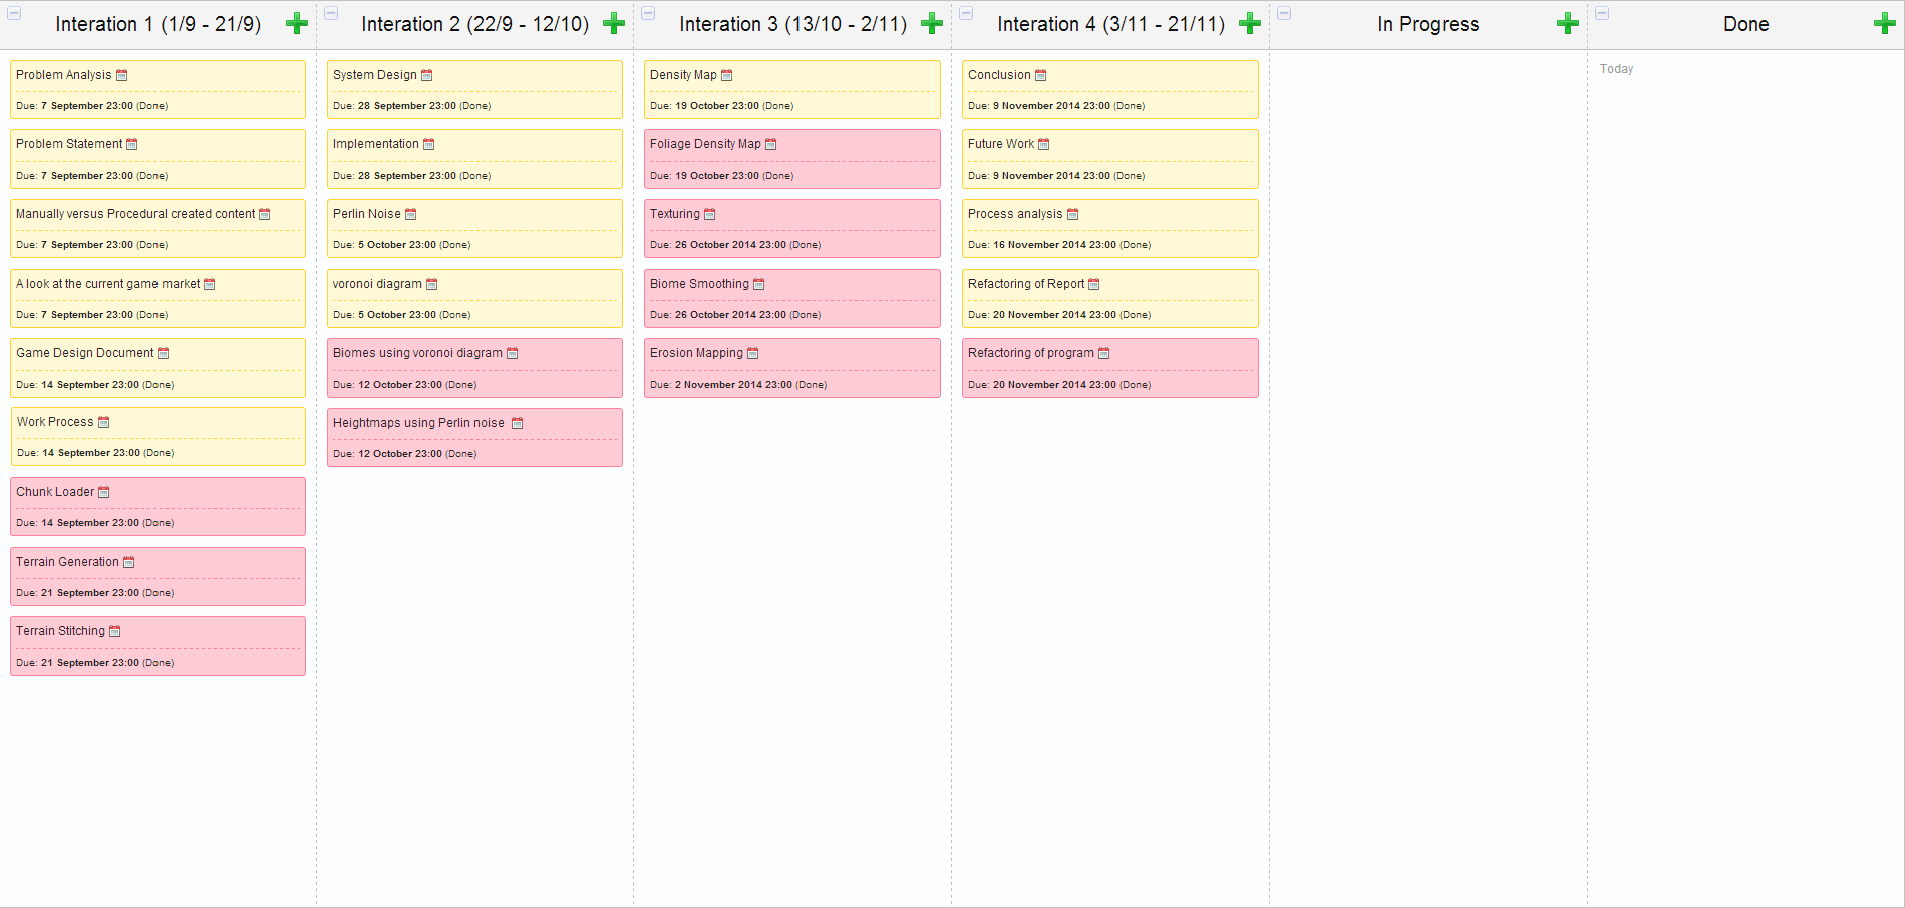
\includegraphics[width=1\linewidth]{img/InitTimeplan}
	\centering
	\caption{The initial time plan created for this project, the yellow blocks means the work is rapport related, where the red blocks are product related.}
	\label{fig:InitTimeplan}
\end{figure}
